\documentclass{article}

\usepackage[letterpaper, portrait, margin=1.5in]{geometry}

\usepackage{fancyhdr}
\usepackage{ragged2e}
\usepackage{graphicx}
\usepackage{caption}
\usepackage{amsmath}
\usepackage{rotating}

\usepackage{listings}
\usepackage{color}

\definecolor{dkgreen}{rgb}{0,0.6,0}
\definecolor{gray}{rgb}{0.5,0.5,0.5}
\definecolor{mauve}{rgb}{0.58,0,0.82}

\lstset{frame=tb,
  language=Java,
  aboveskip=3mm,
  belowskip=3mm,
  showstringspaces=false,
  columns=flexible,
  basicstyle={\small\ttfamily},
  numbers=none,
  numberstyle=\tiny\color{gray},
  keywordstyle=\color{blue},
  commentstyle=\color{dkgreen},
  stringstyle=\color{mauve},
  breaklines=true,
  breakatwhitespace=true,
  tabsize=4
}

\setcounter{secnumdepth}{1}

\usepackage{chngcntr}
\counterwithin{figure}{section}

\renewcommand*{\thepage}{C\arabic{page}}

\pagestyle{fancy}
\lhead{ACME Robotics}
\chead{\#8367}
\rhead{\ifcontents Contents \else Week \thesection \fi}

\newif\ifcontents
\contentstrue

\makeatletter
\renewcommand{\@seccntformat}[1]{}
\makeatother
\begin{document}

\subsection{New Team Marker placement}
%! Find a place to mount the team marker.
After some testing, it was determined that the current placement for the team marker was unreliable. The team marker had previously been placed high on the rear of the robot which caused a great deal of deviation in where the marker landed. Ashlin and Jon were set to this task. They figured that since the problem was that the marker was too high, they would simply put it lower on the robot. This proved to be a little tricky as there was not much space on the lower portion of the robot. The entire right side was taken up by the X-Rail and the left side had both rev hubs on it. The only place that there was space was behind the rev hubs and in front of the lift. Now that they had a place to put it, Ashlin and Jon had to figure out how it would deploy. The original method of deployment (a vertical arm the marker would fall off of when it was swung down) would not work here as there was not enough space. They then came up with the idea of a kicker that push the marker off the side of the robot. They liked this idea because it allowed the servo to sit above the marker, saving space, and it would be more reliable than the previous method. The only problem with this method was that there was nothing stopping the marker from simply falling off the robot. To mediate this problem, Ashlin cut a V shaped fork into the arm that pushed the marker off. The fork could then slide over a section of the marker, holding it in place. This solved the problem, and after some testing the new deployment method worked reliably.

\begin{figure}
    \centering
    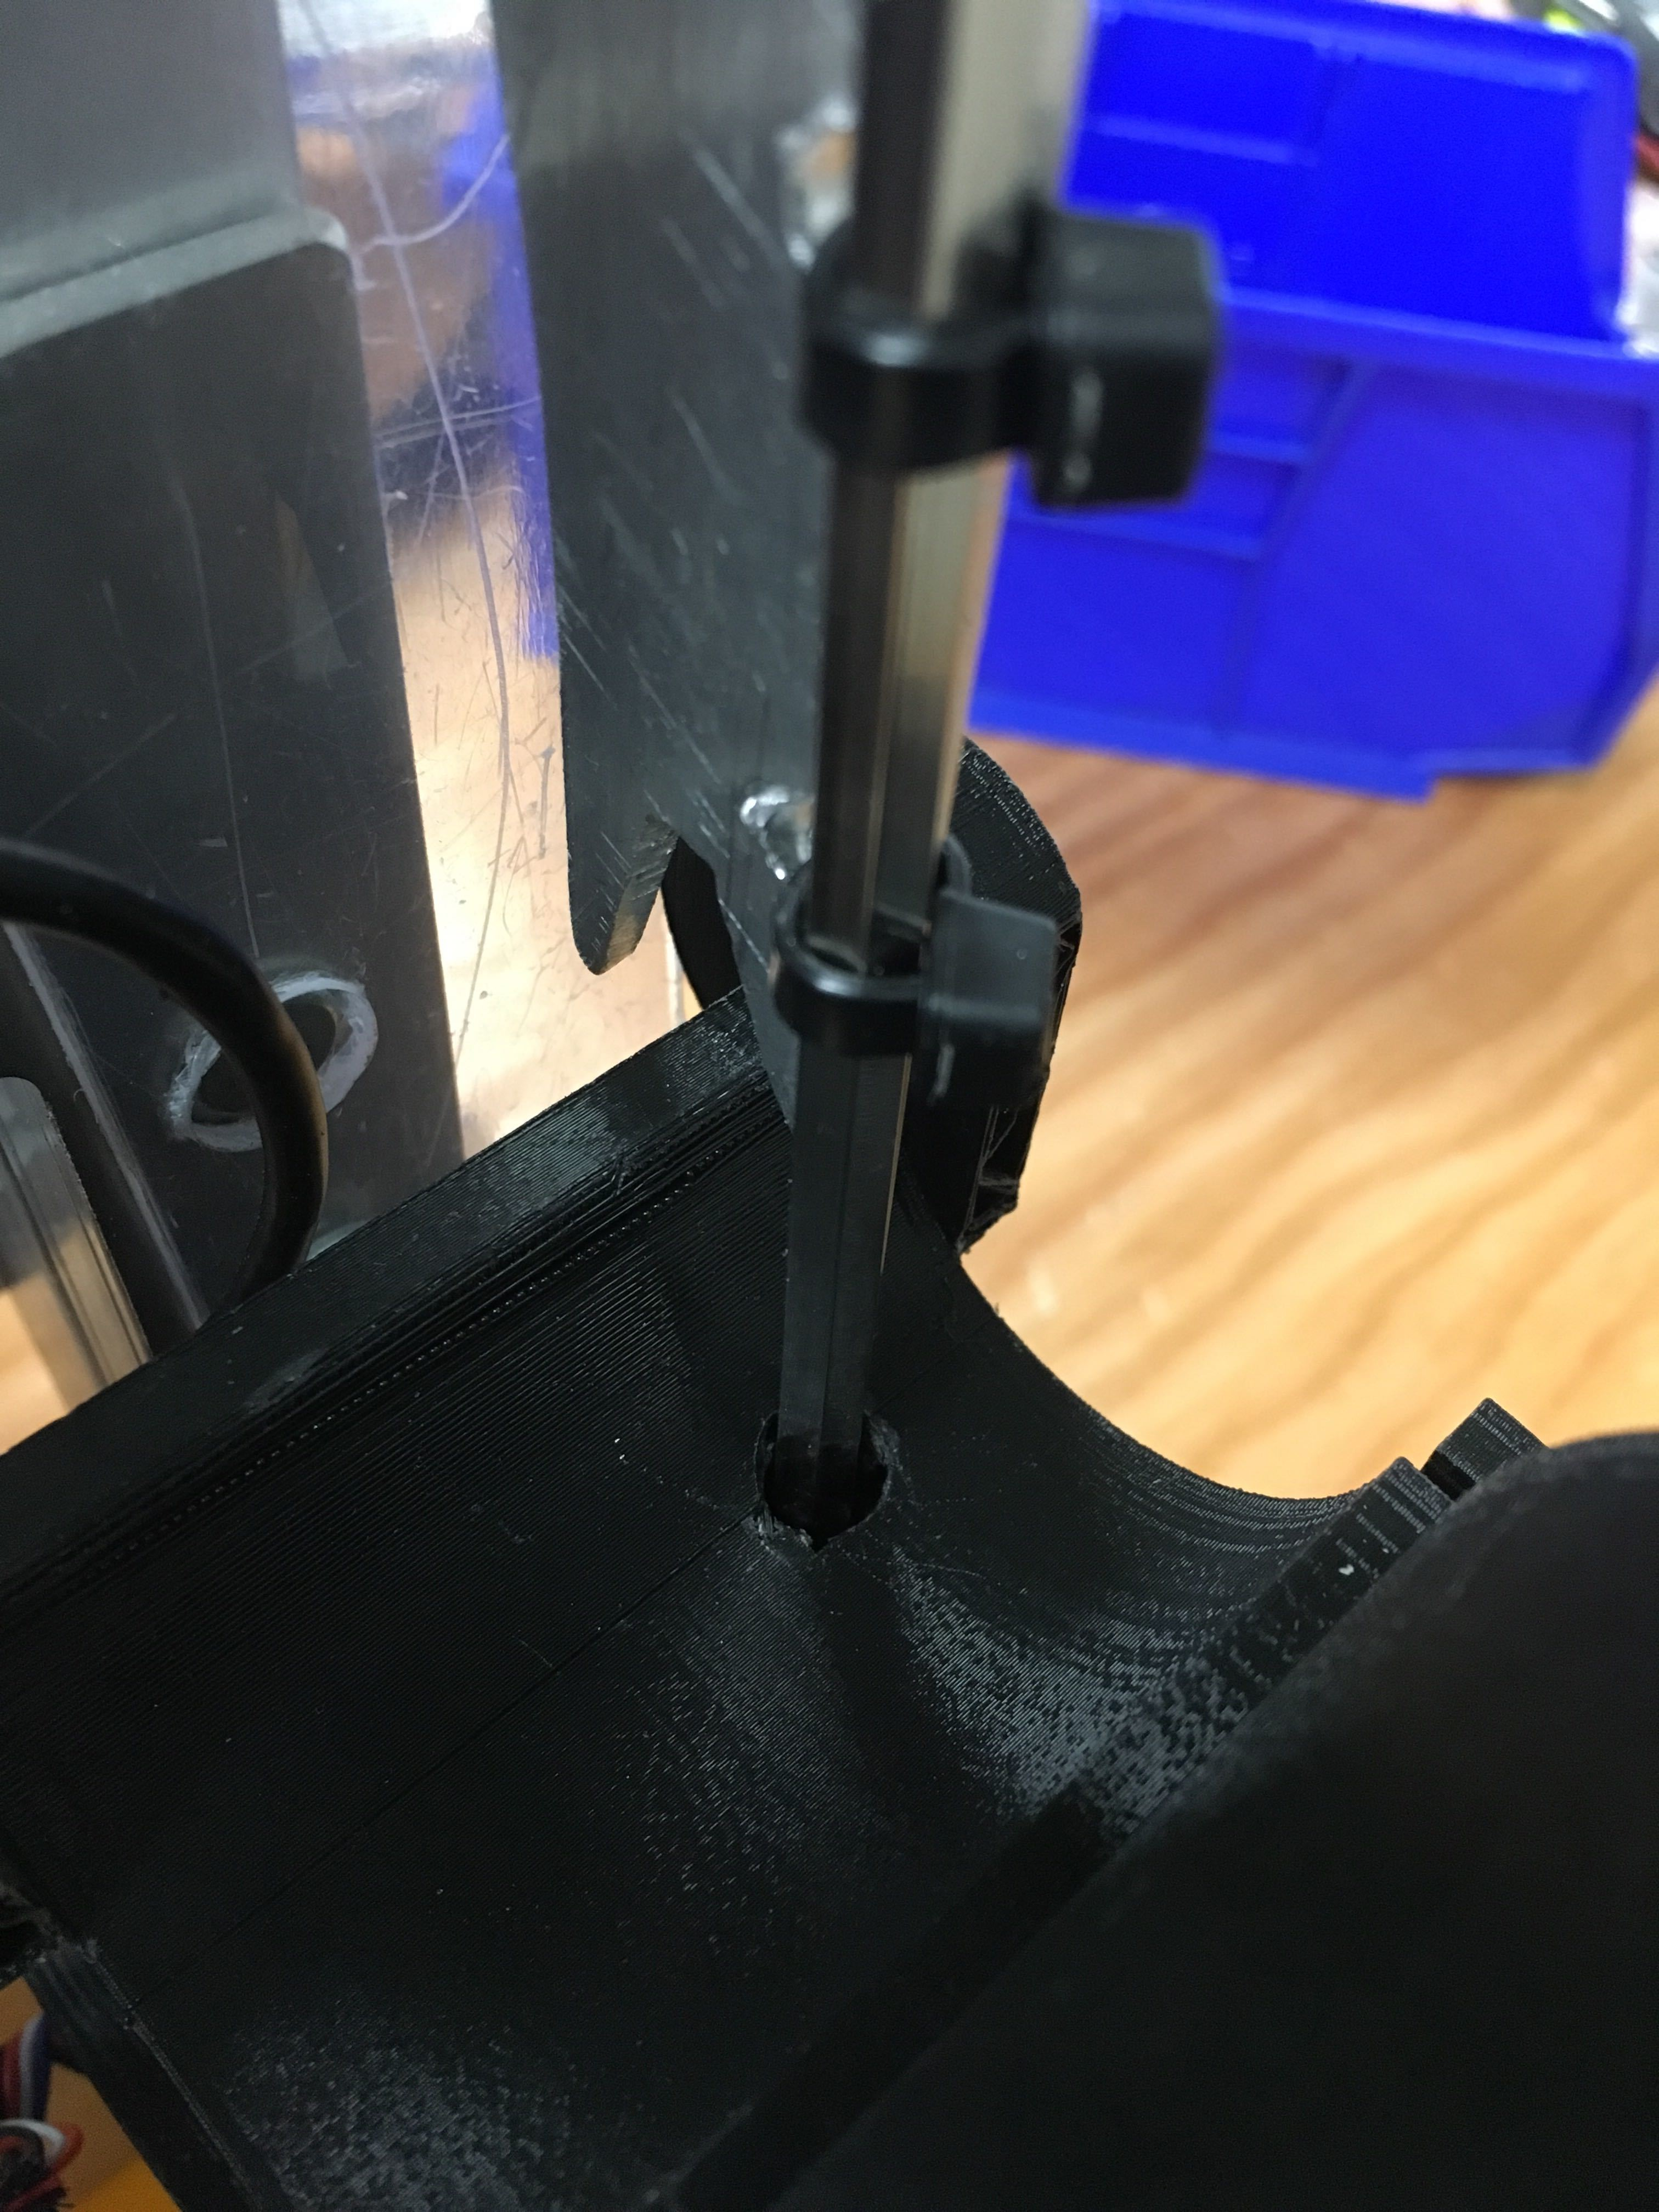
\includegraphics[width=.6 \textwidth]{20_01-14/images/markerplacer.JPG}
    \caption{Marker Placer}
    \label{fig:markerplacer}
\end{figure}

\subsection{Wiring and Rev Hubs}
%! Attaching the Rev Hubs, Battery, phone and wiring the robot.
After most of the subsystems were built the team could then find permanent positions for the rev hubs, battery and phone mount. The team decided to put the rev hubs over the left side wheels because that is where there was the most room and the lowest chance of them getting damaged. To do this Shawn created a poly carbonate sheet that attached to the aluminum side plates and served as a firm attachment place for the rev hubs. Oren then realized that the danger with the rev hubs being there is the chance that wires could get caught in the drive train. To prevent this he created an aluminum plate to attach over the left side drive train to prevent important wires from falling in. Once the rev hubs were mounted the next important thing was to wire all the servos, motors and sensors. The difficult part of this was how to get the wires from the diverter servos because the diverter moved around so much. Kelly fixed this problem by using a wire track that could hold the wires safely inside while matching the up and down motion of the lift. The wires still needed to be run to the other side of the robot and the intake shield attachment bar served as an ideal wire trail from the right side to the left. Once all the wiring was complete the battery and power button were mounted in easily accessible locations and a temporary phone mount was created.

\begin{figure}
    \centering
    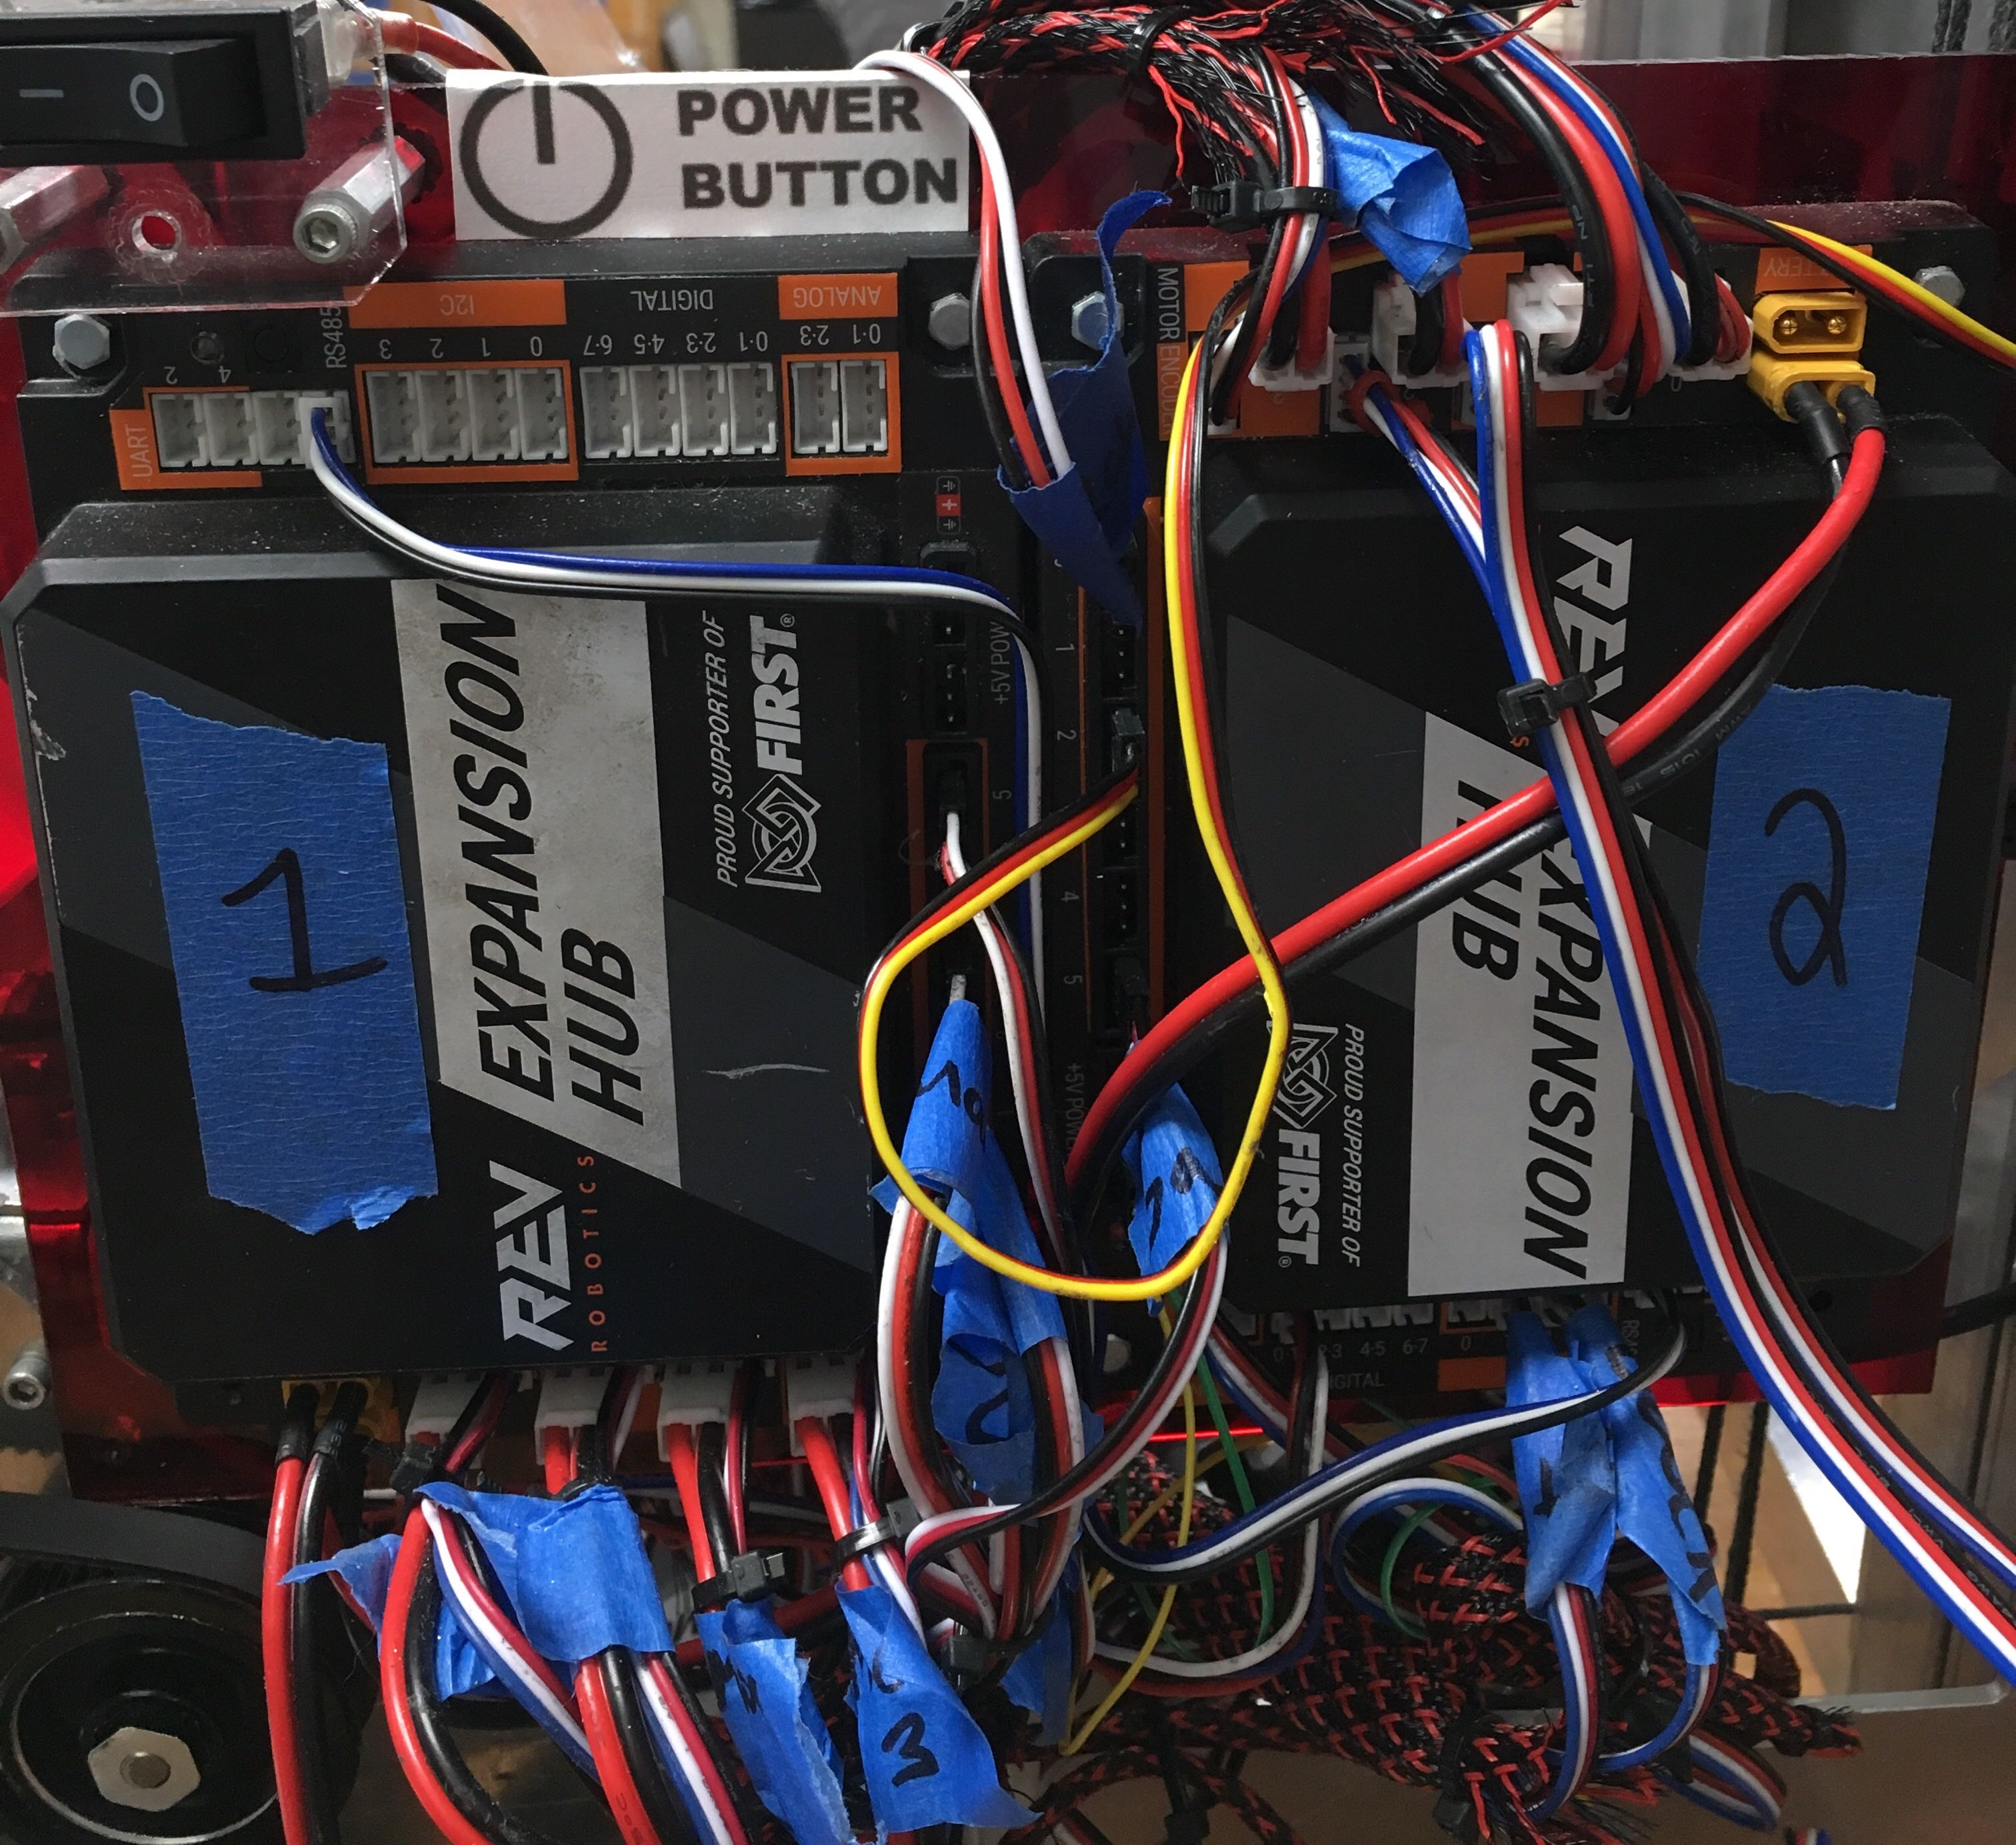
\includegraphics[width=.6 \textwidth]{20_01-14/images/wiring.jpg}
    \caption{Wiring}
    \label{fig:wiring}
\end{figure}

\end{document}